% IA-informed DPS mass mapping, DES Y3-like test: the R(l) kappa forward model against
% NLA alignments built from the density shells, and the effect of ignoring IA in the sampler.
% Build with assets/build_note.sh of the summary-notes skill.
\documentclass[11pt]{article}

\usepackage[margin=1in]{geometry}
\usepackage{amsmath}
\usepackage{amssymb}
\usepackage{graphicx}
\usepackage{booktabs}
\usepackage{xcolor}
\usepackage[font=small,labelfont=bf,labelsep=period]{caption}
\usepackage[hidelinks]{hyperref}

% Symbols, one macro per object.
\newcommand{\T}{^{\mathsf{T}}}
\newcommand{\AIA}{A_{\rm IA}}
\newcommand{\kIA}{\kappa_{\rm IA}}
\newcommand{\Ckk}{C^{\kappa\kappa}}
\newcommand{\CIk}{C^{{\rm I}\kappa}}
\newcommand{\CII}{C^{\rm II}}

% =====================================================================
% Numbers
% =====================================================================
% Every number the text quotes is a macro defined in numbers.tex, which
% make_numbers.py writes from the analysis outputs; each macro there has a
% comment naming its file and key. Part 1: results, refreshed when the
% analysis is rerun (set \numbersfinalfalse to print them in red while
% they are stale). Part 2: inputs.
%
% Statements of the text that rest on Part 1 (re-check after a refresh):
%   - R kappa predicts the same fraction of the IA variance as the theory,
%     in every bin (Summary; "The model reproduces shell-built IA").
%   - The amplitude given the true kappa is unbiased and its error bar is
%     calibrated (Summary; "The model reproduces shell-built IA").
%   - On posterior samples the amplitude statistic returns the amplitude
%     each run assumed ("Posterior samples return the amplitude ...").
%   - Ignoring IA changes the map amplitude at the percent level for DPS
%     and for the tomographic Wiener filter; DPS is positive in all bins,
%     Wiener negative in bins 1 to 3; the single-bin numbers are far
%     larger (Summary; "Ignoring IA changes the maps ...").
%   - "differ by only 2 percent of their rms, yet their A differ by 0.47"
%     and "up to 2.5 percentage points", "three quarters" are typed in
%     the text: re-check them against dps_ia.json after a rerun.
\newif\ifnumbersfinal
\numbersfinaltrue
\newcommand{\refresh}[1]{\ifnumbersfinal#1\else\textcolor{red}{#1}\fi}
% Part 1: results (move when the analysis is rerun).
% des_y3_like/results/validate_ia_model.json, predicted_fraction_measured[0] x 100
\newcommand{\PredFracMeasOne}{\refresh{99.3}}
% des_y3_like/results/validate_ia_model.json, predicted_fraction_theory[0] x 100
\newcommand{\PredFracTheoryOne}{\refresh{99.3}}
% des_y3_like/results/validate_ia_model.json, corr_prediction_with_true_IA[0]
\newcommand{\CorrPredOne}{\refresh{0.996}}
% des_y3_like/results/validate_ia_model.json, rms_ratio_IA_over_kappa[0] (A_IA = 1)
\newcommand{\IAoverKappaOne}{\refresh{0.40}}
% des_y3_like/results/validate_ia_model.json, predicted_fraction_measured[1] x 100
\newcommand{\PredFracMeasTwo}{\refresh{98.9}}
% des_y3_like/results/validate_ia_model.json, predicted_fraction_theory[1] x 100
\newcommand{\PredFracTheoryTwo}{\refresh{98.9}}
% des_y3_like/results/validate_ia_model.json, corr_prediction_with_true_IA[1]
\newcommand{\CorrPredTwo}{\refresh{0.994}}
% des_y3_like/results/validate_ia_model.json, rms_ratio_IA_over_kappa[1] (A_IA = 1)
\newcommand{\IAoverKappaTwo}{\refresh{0.17}}
% des_y3_like/results/validate_ia_model.json, predicted_fraction_measured[2] x 100
\newcommand{\PredFracMeasThree}{\refresh{96.6}}
% des_y3_like/results/validate_ia_model.json, predicted_fraction_theory[2] x 100
\newcommand{\PredFracTheoryThree}{\refresh{96.6}}
% des_y3_like/results/validate_ia_model.json, corr_prediction_with_true_IA[2]
\newcommand{\CorrPredThree}{\refresh{0.983}}
% des_y3_like/results/validate_ia_model.json, rms_ratio_IA_over_kappa[2] (A_IA = 1)
\newcommand{\IAoverKappaThree}{\refresh{0.10}}
% des_y3_like/results/validate_ia_model.json, predicted_fraction_measured[3] x 100
\newcommand{\PredFracMeasFour}{\refresh{71.5}}
% des_y3_like/results/validate_ia_model.json, predicted_fraction_theory[3] x 100
\newcommand{\PredFracTheoryFour}{\refresh{71.5}}
% des_y3_like/results/validate_ia_model.json, corr_prediction_with_true_IA[3]
\newcommand{\CorrPredFour}{\refresh{0.845}}
% des_y3_like/results/validate_ia_model.json, rms_ratio_IA_over_kappa[3] (A_IA = 1)
\newcommand{\IAoverKappaFour}{\refresh{0.07}}
% des_y3_like/results/validate_ia_model.json, max |corr_residual_with_kappa|
\newcommand{\CorrResMax}{\refresh{0.004}}
% des_y3_like/results/validate_ia_model.json, max |spectra_ratio - 1| x 100 over the three spectra, ell > 150
\newcommand{\SpectraDevHighEll}{\refresh{4}}
% des_y3_like/results/validate_ia_model.json, max |spectra_ratio - 1| x 100 over the three spectra, ell < 150
\newcommand{\SpectraDevLowEll}{\refresh{13}}
% des_y3_like/results/validate_ia_model.json, (1 - predicted_fraction_theory[3]) x 100
\newcommand{\ResidFracFour}{\refresh{28}}
% des_y3_like/results/validate_ia_model.json, max |residual_power_ratio - 1| x 100, ell > 150
\newcommand{\ResidualDevHighEll}{\refresh{4}}
% des_y3_like/results/validate_ia_model.json, A_mean
\newcommand{\AmpTruthAllMean}{\refresh{0.53}}
% des_y3_like/results/validate_ia_model.json, A_sem
\newcommand{\AmpTruthAllSem}{\refresh{0.02}}
% des_y3_like/results/validate_ia_model.json, A_reported_sd
\newcommand{\AmpSdPatch}{\refresh{0.23}}
% des_y3_like/results/validate_ia_model.json, A_noiseless_mean
\newcommand{\AmpNoiseless}{\refresh{0.500}}
% des_y3_like/results/validate_ia_model.json, A_noiseless_scatter
\newcommand{\AmpNoiselessScatter}{\refresh{0.001}}
% des_y3_like/results/validate_ia_model.json, pull_std
\newcommand{\PullWidth}{\refresh{0.98}}
% des_y3_like/results/dps_ia.json, summary.n_mocks
\newcommand{\NMocks}{\refresh{4}}
% des_y3_like/results/dps_ia.json, summary.A_given_modelled mean
\newcommand{\AmpGivenModelled}{\refresh{0.53}}
% des_y3_like/results/dps_ia.json, summary.A_given_modelled sem
\newcommand{\AmpGivenModelledSem}{\refresh{0.04}}
% des_y3_like/results/dps_ia.json, summary.A_given_ignored mean
\newcommand{\AmpGivenIgnored}{\refresh{0.07}}
% des_y3_like/results/dps_ia.json, summary.A_given_ignored sem
\newcommand{\AmpGivenIgnoredSem}{\refresh{0.04}}
% des_y3_like/results/dps_ia.json, summary.A_given_truth mean
\newcommand{\AmpGivenTruth}{\refresh{0.32}}
% des_y3_like/results/dps_ia.json, summary.A_given_truth sem
\newcommand{\AmpGivenTruthSem}{\refresh{0.12}}
% des_y3_like/results/dps_ia.json, summary.slope_ratio_minus_1 mean[0] x 100
\newcommand{\BiasOne}{\refresh{\ensuremath{+0.7}}}
% des_y3_like/results/dps_ia.json, summary.slope_ratio_minus_1 sem[0] x 100
\newcommand{\BiasSemOne}{\refresh{0.1}}
% des_y3_like/results/dps_ia.json, summary.slope_modelled mean[0]
\newcommand{\SlopeModelledOne}{\refresh{0.17}}
% des_y3_like/results/dps_ia.json, summary.corr_modelled mean[0]
\newcommand{\CorrModelledOne}{\refresh{0.31}}
% des_y3_like/results/dps_ia.json, summary.corr_ignored mean[0]
\newcommand{\CorrIgnoredOne}{\refresh{0.31}}
% des_y3_like/results/dps_ia.json, summary.corr_KS mean[0]
\newcommand{\CorrKSOne}{\refresh{0.10}}
% des_y3_like/results/dps_ia.json, summary.leak mean[0]
\newcommand{\LeakOne}{\refresh{\ensuremath{-0.00}}}
% des_y3_like/results/dps_ia.json, summary.leak_over_slope mean[0]
\newcommand{\LeakOverSlopeOne}{\refresh{\ensuremath{-0.03}}}
% des_y3_like/results/dps_ia.json, summary.corr_shift_with_IA mean[0]
\newcommand{\ShiftCorrOne}{\refresh{\ensuremath{-0.07}}}
% des_y3_like/results/dps_ia.json, summary.prior_rms_over_truth_rms[0]
\newcommand{\PriorRmsOne}{\refresh{0.98}}
% des_y3_like/results/dps_ia.json, summary.slope_ratio_minus_1 mean[1] x 100
\newcommand{\BiasTwo}{\refresh{\ensuremath{+1.2}}}
% des_y3_like/results/dps_ia.json, summary.slope_ratio_minus_1 sem[1] x 100
\newcommand{\BiasSemTwo}{\refresh{0.1}}
% des_y3_like/results/dps_ia.json, summary.slope_modelled mean[1]
\newcommand{\SlopeModelledTwo}{\refresh{0.21}}
% des_y3_like/results/dps_ia.json, summary.corr_modelled mean[1]
\newcommand{\CorrModelledTwo}{\refresh{0.36}}
% des_y3_like/results/dps_ia.json, summary.corr_ignored mean[1]
\newcommand{\CorrIgnoredTwo}{\refresh{0.37}}
% des_y3_like/results/dps_ia.json, summary.corr_KS mean[1]
\newcommand{\CorrKSTwo}{\refresh{0.19}}
% des_y3_like/results/dps_ia.json, summary.leak mean[1]
\newcommand{\LeakTwo}{\refresh{\ensuremath{-0.01}}}
% des_y3_like/results/dps_ia.json, summary.leak_over_slope mean[1]
\newcommand{\LeakOverSlopeTwo}{\refresh{\ensuremath{-0.06}}}
% des_y3_like/results/dps_ia.json, summary.corr_shift_with_IA mean[1]
\newcommand{\ShiftCorrTwo}{\refresh{\ensuremath{-0.06}}}
% des_y3_like/results/dps_ia.json, summary.prior_rms_over_truth_rms[1]
\newcommand{\PriorRmsTwo}{\refresh{0.98}}
% des_y3_like/results/dps_ia.json, summary.slope_ratio_minus_1 mean[2] x 100
\newcommand{\BiasThree}{\refresh{\ensuremath{+1.8}}}
% des_y3_like/results/dps_ia.json, summary.slope_ratio_minus_1 sem[2] x 100
\newcommand{\BiasSemThree}{\refresh{0.1}}
% des_y3_like/results/dps_ia.json, summary.slope_modelled mean[2]
\newcommand{\SlopeModelledThree}{\refresh{0.23}}
% des_y3_like/results/dps_ia.json, summary.corr_modelled mean[2]
\newcommand{\CorrModelledThree}{\refresh{0.39}}
% des_y3_like/results/dps_ia.json, summary.corr_ignored mean[2]
\newcommand{\CorrIgnoredThree}{\refresh{0.39}}
% des_y3_like/results/dps_ia.json, summary.corr_KS mean[2]
\newcommand{\CorrKSThree}{\refresh{0.27}}
% des_y3_like/results/dps_ia.json, summary.leak mean[2]
\newcommand{\LeakThree}{\refresh{\ensuremath{-0.01}}}
% des_y3_like/results/dps_ia.json, summary.leak_over_slope mean[2]
\newcommand{\LeakOverSlopeThree}{\refresh{\ensuremath{-0.04}}}
% des_y3_like/results/dps_ia.json, summary.corr_shift_with_IA mean[2]
\newcommand{\ShiftCorrThree}{\refresh{\ensuremath{-0.03}}}
% des_y3_like/results/dps_ia.json, summary.prior_rms_over_truth_rms[2]
\newcommand{\PriorRmsThree}{\refresh{0.99}}
% des_y3_like/results/dps_ia.json, summary.slope_ratio_minus_1 mean[3] x 100
\newcommand{\BiasFour}{\refresh{\ensuremath{+3.0}}}
% des_y3_like/results/dps_ia.json, summary.slope_ratio_minus_1 sem[3] x 100
\newcommand{\BiasSemFour}{\refresh{0.1}}
% des_y3_like/results/dps_ia.json, summary.slope_modelled mean[3]
\newcommand{\SlopeModelledFour}{\refresh{0.23}}
% des_y3_like/results/dps_ia.json, summary.corr_modelled mean[3]
\newcommand{\CorrModelledFour}{\refresh{0.38}}
% des_y3_like/results/dps_ia.json, summary.corr_ignored mean[3]
\newcommand{\CorrIgnoredFour}{\refresh{0.39}}
% des_y3_like/results/dps_ia.json, summary.corr_KS mean[3]
\newcommand{\CorrKSFour}{\refresh{0.32}}
% des_y3_like/results/dps_ia.json, summary.leak mean[3]
\newcommand{\LeakFour}{\refresh{\ensuremath{-0.04}}}
% des_y3_like/results/dps_ia.json, summary.leak_over_slope mean[3]
\newcommand{\LeakOverSlopeFour}{\refresh{\ensuremath{-0.19}}}
% des_y3_like/results/dps_ia.json, summary.corr_shift_with_IA mean[3]
\newcommand{\ShiftCorrFour}{\refresh{\ensuremath{-0.07}}}
% des_y3_like/results/dps_ia.json, summary.prior_rms_over_truth_rms[3]
\newcommand{\PriorRmsFour}{\refresh{0.99}}
% des_y3_like/results/dps_ia.json, summary.rms_shift_over_rms_mean, mean over bins x 100
\newcommand{\RmsShiftPercent}{\refresh{3}}
% des_y3_like/results/wiener_reference.json, slope_ratio_minus_1 mean[0] x 100
\newcommand{\WFBiasOne}{\refresh{\ensuremath{-1.2}}}
% des_y3_like/results/wiener_reference_deep.json, slope_ratio_minus_1 mean[0] x 100
\newcommand{\WFDeepBiasOne}{\refresh{\ensuremath{-3.3}}}
% des_y3_like/results/wiener_reference.json, single_bin_slope_ratio_minus_1 mean[0] x 100
\newcommand{\WFSingleBiasOne}{\refresh{\ensuremath{+15.4}}}
% des_y3_like/results/wiener_reference.json, slope_modelled mean[0]
\newcommand{\WFSlopeOne}{\refresh{0.23}}
% des_y3_like/results/wiener_reference.json, corr_modelled mean[0]
\newcommand{\WFCorrOne}{\refresh{0.48}}
% des_y3_like/results/wiener_reference.json, slope_ratio_minus_1 mean[1] x 100
\newcommand{\WFBiasTwo}{\refresh{\ensuremath{-0.8}}}
% des_y3_like/results/wiener_reference_deep.json, slope_ratio_minus_1 mean[1] x 100
\newcommand{\WFDeepBiasTwo}{\refresh{\ensuremath{-2.4}}}
% des_y3_like/results/wiener_reference.json, single_bin_slope_ratio_minus_1 mean[1] x 100
\newcommand{\WFSingleBiasTwo}{\refresh{\ensuremath{+2.9}}}
% des_y3_like/results/wiener_reference.json, slope_modelled mean[1]
\newcommand{\WFSlopeTwo}{\refresh{0.28}}
% des_y3_like/results/wiener_reference.json, corr_modelled mean[1]
\newcommand{\WFCorrTwo}{\refresh{0.53}}
% des_y3_like/results/wiener_reference.json, slope_ratio_minus_1 mean[2] x 100
\newcommand{\WFBiasThree}{\refresh{\ensuremath{-0.2}}}
% des_y3_like/results/wiener_reference_deep.json, slope_ratio_minus_1 mean[2] x 100
\newcommand{\WFDeepBiasThree}{\refresh{\ensuremath{-1.4}}}
% des_y3_like/results/wiener_reference.json, single_bin_slope_ratio_minus_1 mean[2] x 100
\newcommand{\WFSingleBiasThree}{\refresh{\ensuremath{+0.5}}}
% des_y3_like/results/wiener_reference.json, slope_modelled mean[2]
\newcommand{\WFSlopeThree}{\refresh{0.30}}
% des_y3_like/results/wiener_reference.json, corr_modelled mean[2]
\newcommand{\WFCorrThree}{\refresh{0.55}}
% des_y3_like/results/wiener_reference.json, slope_ratio_minus_1 mean[3] x 100
\newcommand{\WFBiasFour}{\refresh{\ensuremath{+0.5}}}
% des_y3_like/results/wiener_reference_deep.json, slope_ratio_minus_1 mean[3] x 100
\newcommand{\WFDeepBiasFour}{\refresh{\ensuremath{-0.5}}}
% des_y3_like/results/wiener_reference.json, single_bin_slope_ratio_minus_1 mean[3] x 100
\newcommand{\WFSingleBiasFour}{\refresh{\ensuremath{+0.3}}}
% des_y3_like/results/wiener_reference.json, slope_modelled mean[3]
\newcommand{\WFSlopeFour}{\refresh{0.30}}
% des_y3_like/results/wiener_reference.json, corr_modelled mean[3]
\newcommand{\WFCorrFour}{\refresh{0.55}}
% des_y3_like/results/wiener_reference_deep.json, neff
\newcommand{\DeepNEff}{7.5}
% notes/des_y3_like_ia/plots/dps_response/data.json, ks_bias_percent[0]
\newcommand{\KSBiasOne}{\refresh{\ensuremath{-17.6}}}
% notes/des_y3_like_ia/plots/dps_response/data.json, ks_bias_percent[1]
\newcommand{\KSBiasTwo}{\refresh{\ensuremath{-5.4}}}
% notes/des_y3_like_ia/plots/dps_response/data.json, ks_bias_percent[2]
\newcommand{\KSBiasThree}{\refresh{\ensuremath{-1.6}}}
% notes/des_y3_like_ia/plots/dps_response/data.json, ks_bias_percent[3]
\newcommand{\KSBiasFour}{\refresh{\ensuremath{-1.3}}}
% des_y3_like/results/toy_and_checks.json, toy_A_truth
\newcommand{\ToyAmpTruth}{\refresh{0.61}}
% des_y3_like/results/toy_and_checks.json, toy_A_truth_sd
\newcommand{\ToyAmpTruthSd}{\refresh{0.06}}
% des_y3_like/results/toy_and_checks.json, toy_A_modelled
\newcommand{\ToyAmpModelled}{\refresh{0.51}}
% des_y3_like/results/toy_and_checks.json, toy_A_ignored
\newcommand{\ToyAmpIgnored}{\refresh{0.10}}
% des_y3_like/results/toy_and_checks.json, roman_spurious_max
\newcommand{\RomanSpuriousMax}{\refresh{1.3}}
% des_y3_like/results/toy_and_checks.json, train_minutes
\newcommand{\TrainMinutes}{\refresh{40}}
% des_y3_like/results/toy_and_checks.json, sample_minutes_per_run
\newcommand{\SampleMinutes}{\refresh{5}}
% des_y3_like/results/toy_and_checks.json, shells_vs_ccl_des_percent
\newcommand{\ShellsVsCCLDes}{\refresh{0.5}}
% des_y3_like/results/toy_and_checks.json, shells_vs_ccl_roman_percent
\newcommand{\ShellsVsCCLRoman}{\refresh{0.3}}
% Part 2: inputs (a rerun does not change them).
% work/maps_info.json, npix
\newcommand{\NPix}{64}
% work/maps_info.json, pixel_arcmin
\newcommand{\PixArcmin}{8}
% work/maps_info.json, theta_max_deg
\newcommand{\FieldDeg}{8.53}
% work/maps_info.json, n_shells
\newcommand{\NShells}{100}
% work/maps_info.json, n_shells_shifted
\newcommand{\NShellsShifted}{58}
% work/maps_info.json, z_max
\newcommand{\ZMax}{3.0}
% work/maps_info.json, n_train
\newcommand{\NTrain}{4000}
% work/maps_info.json, n_test
\newcommand{\NTest}{100}
% work/maps_info.json, cosmology.Omega_c
\newcommand{\OmegaC}{0.25}
% work/maps_info.json, cosmology.Omega_b
\newcommand{\OmegaB}{0.05}
% work/maps_info.json, cosmology.h
\newcommand{\Hubble}{0.68}
% work/maps_info.json, cosmology.sigma8
\newcommand{\SigmaEight}{0.81}
% work/maps_info.json, cosmology.n_s
\newcommand{\SpectralIndex}{0.965}
% work/maps_info.json, kappa_rms[0] x 1000
\newcommand{\KappaRmsOne}{3.1}
% work/maps_info.json, kappa_rms[1] x 1000
\newcommand{\KappaRmsTwo}{5.2}
% work/maps_info.json, kappa_rms[2] x 1000
\newcommand{\KappaRmsThree}{7.8}
% work/maps_info.json, kappa_rms[3] x 1000
\newcommand{\KappaRmsFour}{9.4}
% work/maps_info.json, shell_var_delta_max
\newcommand{\ShellVarMax}{12}
% des_y3_like/des_like.yaml, train.nsteps
\newcommand{\TrainSteps}{2000}
% DPS_mass_mapping train.py, train_batch_size
\newcommand{\TrainBatch}{24}
% DPS_mass_mapping train.py, Unet dim
\newcommand{\UnetWidth}{64}
% des_y3_like/run_des_like.py, --delta_t default
\newcommand{\DeltaT}{500}
% des_y3_like/run_des_like.py, --sigma_t default
\newcommand{\SigmaT}{20}
% des_y3_like/run_des_like.py, --steps default
\newcommand{\SampleSteps}{1000}
% des_y3_like/run_des_like.py, --n_samples default
\newcommand{\NSamples}{4}
% des_y3_like/des_like.yaml, ia.A_IA
\newcommand{\AInjected}{0.5}
% des_y3_like/results/validate_ia_model.json, sigma_pixel
\newcommand{\SigmaPixel}{0.027}
% des_y3_like/des_like.yaml, data.neff
\newcommand{\NEff}{1.475}
% des_y3_like/des_like.yaml, data.sigma_e
\newcommand{\SigmaE}{0.26}


\begin{document}

\begin{center}
  {\LARGE IA-informed DPS mass mapping: a DES Y3-like test\par}
  \vspace{0.6em}
  {\large Does the $R(\ell)\,\kappa$ forward model describe field-level NLA alignments,
  and what does a sampler that ignores them do?\par}
  \vspace{0.6em}
  {\large November 2026\par}
  \ifnumbersfinal\else
    \vspace{0.6em}
    {\color{red}Numbers in red are being refreshed.\par}
  \fi
\end{center}
\vspace{1em}

\section{Summary}
\label{sec:summary}

\paragraph{The question.}
Real DES Y3 shear contains intrinsic alignments (IA), and the DPS mass-mapping code assumes
none. Does the IA forward model added to the sampler, $\kappa \rightarrow \kappa + \AIA R(\ell)\kappa$,
describe NLA alignments that are built independently at field level, and how much does a
DES Y3-like DPS reconstruction change when IA is ignored?

\paragraph{The answer.}
The model describes shell-built NLA IA to the precision of the test: $R\kappa$ predicts
\PredFracMeasOne, \PredFracMeasTwo, \PredFracMeasThree\ and \PredFracMeasFour\ percent of the IA
variance in bins 1 to 4, equal to the theory values, and the injected $\AIA = \AInjected$ is
recovered as \AmpNoiseless\ without noise and $\AmpTruthAllMean \pm \AmpTruthAllSem$ at DES Y3
noise when the true $\kappa$ is given. At DES Y3 depth the effect of ignoring IA on the maps is
at the percent level: the DPS posterior mean moves by about \RmsShiftPercent\ percent of its rms
and its amplitude changes by \BiasOne, \BiasTwo, \BiasThree\ and \BiasFour\ percent in bins 1 to
4; the tomographic Wiener filter, the linear reference, gives \WFBiasOne, \WFBiasTwo,
\WFBiasThree\ and \WFBiasFour\ percent.

\paragraph{Why.}
$R$ is the least-squares projection of the IA weights of Eq.~(\ref{eq:shells}) on the four
lensing weights, so $R\kappa$ is the best prediction of the IA that four lensing maps allow,
and what it leaves out is uncorrelated with $\kappa$ (Section~\ref{sec:model}, The model
reproduces shell-built IA). The maps barely react to IA because bins 1 and 2, where IA is
large, are noise dominated: their maps are set mostly by the prior's correlation with bins 3
and 4, whose IA is small. A noise-free single-bin estimate gives \KSBiasOne\ percent in bin 1,
and a Wiener filter that uses bin 1 alone \WFSingleBiasOne\ percent; neither applies to a
joint tomographic reconstruction at this depth (Section~\ref{sec:maps}, Ignoring IA changes
the maps at the percent level).

\paragraph{Limits.}
The maps are lognormal shells with bounded skewness at \PixArcmin\ arcmin pixels, not an
$N$-body simulation and not DES Y3 data. The DPS numbers come from \NMocks\ mocks with
\NSamples\ samples each. DPS and the Wiener filter differ by up to 2.5 percentage points in the
amplitude change, with opposite signs in bins 1 to 3, and the DPS response to the true signal
is about three quarters of the Wiener one; both are listed in Section~\ref{app:open}, Open
issues. The IA amplitude evaluated on posterior samples returns the amplitude the sampler
assumed and is not a measurement (Section~\ref{sec:amp}, Posterior samples return the
amplitude of their own forward model).

\section{Setup and definitions}
\label{sec:setup}

\paragraph{Maps.}
The lightcone to $z = \ZMax$ is cut into \NShells\ shells of equal comoving width. Shell $i$
carries a density contrast $\delta_i(\boldsymbol\theta)$ with the Limber spectrum of a thin shell,
\begin{equation}
  C_i(\ell) = \frac{P_{\rm nl}\!\left(k = (\ell + 1/2)/\chi_i,\, z_i\right)}{\chi_i^2\,\Delta\chi_i} ,
\end{equation}
and the maps of source bin $b$ are weighted sums over the same shells:
\begin{equation}
  \kappa_b = \sum_i W_{b,i}\,\delta_i , \qquad
  \kappa_{{\rm IA},b} = \sum_i w_{b,i}\,\delta_i , \qquad
  w_{b,i} = -F(z_i)\, f_{b,i} .
  \label{eq:shells}
\end{equation}
$W_{b,i}$ is the lensing efficiency of bin $b$ times the shell width, $f_{b,i}$ the fraction of
bin-$b$ sources inside shell $i$, and
$F(z) = \AIA\, C_1\rho_{\rm crit}\,\Omega_m / D(z)$ with $C_1\rho_{\rm crit} = 0.0139$ and
$D(0) = 1$ (the NLA convention of CCL). $\kIA$ is stored at $\AIA = 1$. This is the
construction of the repository's training patches, with lognormal shells in place of the
particle shells of an $N$-body simulation; \texttt{nla\_shell\_weights.py} gives both sets of
weights. Each $\delta_i$ is a shifted lognormal field whose skewness is bounded (Section
\ref{app:method}, Method details).

\paragraph{Fiducial values.}
Source redshift distributions: the four DES Y3 bins, from the Cocoa file
{\small\texttt{nz\_source\_Y3\_unblinded\_02\_26\_21.txt}}.

\noindent Cosmology: $\Omega_c = \OmegaC$,
$\Omega_b = \OmegaB$, $h = \Hubble$, $\sigma_8 = \SigmaEight$, $n_s = \SpectralIndex$, Halofit.
Grid: $\NPix \times \NPix$ pixels of \PixArcmin\ arcmin, a field of \FieldDeg\ degrees, the size
of the DES Y3 data patches of the repository (which use 2 arcmin pixels). The rms of $\kappa$
per pixel is $(\KappaRmsOne, \KappaRmsTwo, \KappaRmsThree, \KappaRmsFour) \times 10^{-3}$ in
bins 1 to 4. Shape noise: $\sigma_e = \SigmaE$ per component and \NEff\ galaxies per
arcmin$^2$ per bin, which gives $\sigma = \SigmaPixel$ per pixel and component. The mocks
contain IA with $\AIA = \AInjected$:
shear $= {\rm KS}\left[\kappa + \AIA\,\kIA\right] +$ noise, with KS the flat-sky
Kaiser-Squires forward operator of the repository.

\paragraph{The IA forward model.}
The sampler does not know $\delta_i$. It models the IA of bin $b$ from the four convergence
maps it is inferring,
\begin{equation}
  \kappa_{{\rm IA},b}(\boldsymbol\ell) = \sum_c R_{bc}(\ell)\,\kappa_c(\boldsymbol\ell) + \epsilon_b(\boldsymbol\ell),
  \qquad R = \CIk\,[\Ckk]^{-1}, \qquad S = \CII - R\,\Ckk R\T ,
  \label{eq:model}
\end{equation}
where $\Ckk$, $\CIk$ and $\CII$ are the $4 \times 4$ Limber spectra at $\AIA = 1$, $R\kappa$ is
the part of the IA that the lensing maps predict, and $\epsilon$ is the remainder, uncorrelated
with $\kappa$, with spectrum $S$. The forward model of the sampler is
${\rm KS}\left[\kappa + \AIA R\kappa\right]$ (\texttt{ia\_forward.py}); $\epsilon$ is not in the
likelihood. The spectra are those of the same shells as the maps
(\texttt{work/ia\_spectra\_shells.npz}).

\paragraph{Prior and sampler.}
The diffusion prior is the U-Net of the repository (base width \UnetWidth), trained for \TrainSteps\ steps
with batch size \TrainBatch\ on \NTrain\ maps; \NTest\ further maps are held out. Posterior samples use
the repository's default guidance (\texttt{dps\_sigmoid}, $\delta_t = \DeltaT$, $\sigma_t = \SigmaT$,
\SampleSteps\ steps), \NSamples\ samples per run. For each mock two runs use the same data and the same random seed, one with
$\AIA = \AInjected$ in the forward model (``IA modelled'') and one with $\AIA = 0$ (``IA
ignored''), so their difference is the effect of the IA term and not sampling scatter.

\paragraph{Statistics.}
With $t$ the true $\kappa$ of a bin and $m$ a posterior mean, both with their means removed,
the \emph{slope} is $\langle m\,t\rangle / \langle t\,t\rangle$, the response of the posterior
mean to the true signal. The \emph{amplitude preferred by the data given a map} is the mean of
the exact Gaussian conditional $p(\AIA \mid \kappa, {\rm data})$, which exists because the shear
is linear in $\AIA$ at fixed $\kappa$:
\begin{equation}
  \hat A = \frac{\sum w\,({\rm data} - {\rm KS}[\kappa]) \cdot {\rm KS}[R\kappa]}
                {\sum w\,|{\rm KS}[R\kappa]|^2},
  \qquad \sigma_A = \Big(\sum w\,|{\rm KS}[R\kappa]|^2\Big)^{-1/2},
  \label{eq:amp}
\end{equation}
with $w = 1/\sigma^2$ and the sums over pixels, shear components and bins.

\section{The model reproduces shell-built IA}
\label{sec:model}

$R\kappa$ accounts for the IA maps exactly as the two-point theory says it can. On the \NTest\
held-out maps, with no noise and no sampler, the fraction of the variance of $\kIA$ removed by
subtracting $R\kappa$ is \PredFracMeasOne, \PredFracMeasTwo, \PredFracMeasThree\ and
\PredFracMeasFour\ percent in bins 1 to 4, against \PredFracTheoryOne, \PredFracTheoryTwo,
\PredFracTheoryThree\ and \PredFracTheoryFour\ percent from the spectra. The remainder is
uncorrelated with $\kappa$ (correlation coefficient below \CorrResMax\ in every bin) and its
power follows the model spectrum $S$ (Figure~\ref{fig:model}). Bin 4 is the least predictable
because its sources sit behind most of the matter that lenses the other bins, so no
combination of lensing maps isolates the matter at $z \approx 1$.

The amplitude of Eq.~(\ref{eq:amp}), evaluated with the true $\kappa$, is unbiased: without
noise $\hat A = \AmpNoiseless$ with a scatter of \AmpNoiselessScatter\ between maps, which is the
whole effect of the part $\epsilon$ that the model leaves out. With DES Y3 noise the mean over
the \NTest\ maps is $\AmpTruthAllMean \pm \AmpTruthAllSem$ and one \FieldDeg\ degree patch
constrains $\AIA$ to $\pm\AmpSdPatch$.

\begin{figure}[tbp]
  \centering
  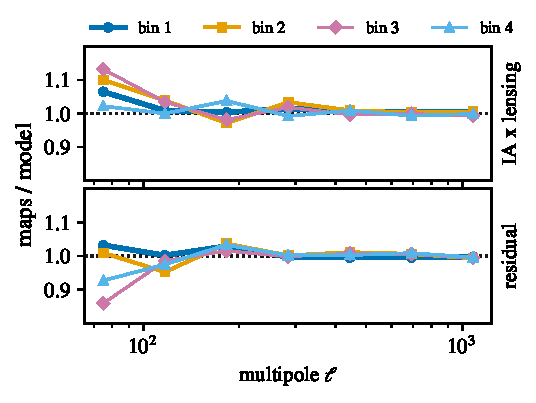
\includegraphics[width=3.5in]{plots/ia_model_test/ia_model_test.pdf}
  \caption{Shell-built IA maps against the model, on the held-out maps. Top: measured
  $\CIk$ of each source bin over its Limber spectrum. Bottom: power of $\kIA - R\kappa$ over
  the model spectrum $S$. Color, line width and marker: the source bin; dotted: maps and model
  agree. The lowest multipole bins hold few modes.}
  \label{fig:model}
\end{figure}

\section{Posterior samples return the amplitude of their own forward model}
\label{sec:amp}

Evaluated on posterior samples, $\hat A$ is $\AmpGivenModelled \pm \AmpGivenModelledSem$ for the
run with the IA model and $\AmpGivenIgnored \pm \AmpGivenIgnoredSem$ for the run without it
(Figure~\ref{fig:amp}), which are the amplitudes \AInjected\ and 0 that the two runs assumed.
The reason is in the sampler: a sample of the run with forward model
${\rm KS}[\kappa + A_{\rm m} R\kappa]$ leaves a residual
$r = {\rm data} - {\rm KS}[\kappa + A_{\rm m} R\kappa]$ that the likelihood gradient has made
uncorrelated with the template ${\rm KS}[R\kappa]$, so
${\rm data} - {\rm KS}[\kappa] = r + A_{\rm m}\,{\rm KS}[R\kappa]$ projects onto the template
with coefficient $A_{\rm m}$. The paired samples of the two runs differ by only 2 percent of
their rms, yet their $\hat A$ differ by $0.47$. On posterior samples the statistic is
therefore a consistency check of the sampler, not a measurement of $\AIA$ and not evidence of
IA absorbed into the maps. Given the true $\kappa$ of the same \NMocks\ mocks it is
$\AmpGivenTruth \pm \AmpGivenTruthSem$.

\begin{figure}[tbp]
  \centering
  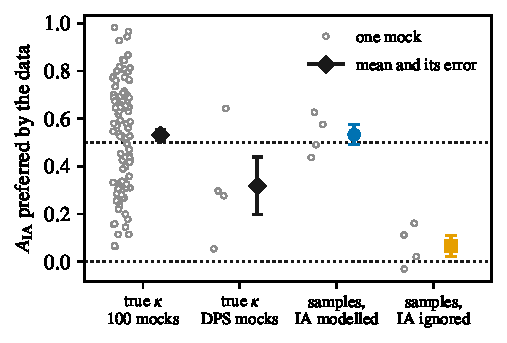
\includegraphics[width=3.5in]{plots/ia_amplitude/ia_amplitude.pdf}
  \caption{The IA amplitude $\hat A$ of Eq.~(\ref{eq:amp}) for different choices of the map
  it is conditioned on: the true $\kappa$ of the held-out maps, the true $\kappa$ of the mocks
  sampled with DPS, and the posterior samples of the two DPS runs. Open circles: one mock;
  filled symbols: the mean and its standard error; dotted: the injected amplitude and zero.}
  \label{fig:amp}
\end{figure}

\section{Ignoring IA changes the maps at the percent level}
\label{sec:maps}

At DES Y3 noise the reconstructed maps are almost the same with and without the IA term. The
posterior means of the two runs differ by \RmsShiftPercent\ percent of their rms, and the slope
of the posterior mean against the truth changes by \BiasOne, \BiasTwo, \BiasThree\ and
\BiasFour\ percent in bins 1 to 4 when IA is ignored (Figure~\ref{fig:response}; the standard
error over the mocks is \BiasSemOne\ percent, small because the two runs share their random
numbers). The shift is not a copy of the injected IA: its slope against $\AIA\kIA$ is
\LeakOne, \LeakTwo, \LeakThree\ and \LeakFour\ (Figure~\ref{fig:maps}).

The tomographic Wiener filter, which is the posterior mean for Gaussian fields with the same
spectra, gives the same order of magnitude: \WFBiasOne, \WFBiasTwo, \WFBiasThree\ and
\WFBiasFour\ percent. The same filter restricted to one bin changes by \WFSingleBiasOne\
percent in bin 1, so the insensitivity comes from the tomography: the noise per pixel is
\SigmaPixel\ against a signal rms of $\KappaRmsOne \times 10^{-3}$ in bin 1, the map of bin 1 is
reconstructed mostly from the bins behind it through the prior, and those bins carry little IA
(the rms of $\kIA$ at $\AIA = 1$ is \IAoverKappaOne, \IAoverKappaTwo, \IAoverKappaThree\ and
\IAoverKappaFour\ of the rms of $\kappa$ in bins 1 to 4). The sign of the single-bin number is
also instructive: in the noise-dominated regime a filter that knows the signal is suppressed
by IA weights the data \emph{less}, so modelling IA lowers the amplitude of the estimate, the
opposite of the noise-free expectation of \KSBiasOne\ percent. With \DeepNEff\ galaxies per
arcmin$^2$ per bin the tomographic Wiener change grows to \WFDeepBiasOne, \WFDeepBiasTwo,
\WFDeepBiasThree\ and \WFDeepBiasFour\ percent.

The DPS reconstruction itself behaves as a tomographic reconstruction at this depth: the
prior samples have \PriorRmsOne\ to \PriorRmsFour\ of the true rms, and the posterior mean
correlates with the truth at \CorrModelledOne, \CorrModelledTwo, \CorrModelledThree\ and
\CorrModelledFour\ in bins 1 to 4, against \CorrKSOne, \CorrKSTwo, \CorrKSThree\ and
\CorrKSFour\ for the Kaiser-Squires map. Its slope against the truth is \SlopeModelledOne,
\SlopeModelledTwo, \SlopeModelledThree\ and \SlopeModelledFour, below the Wiener values
\WFSlopeOne, \WFSlopeTwo, \WFSlopeThree\ and \WFSlopeFour.

\begin{figure}[tbp]
  \centering
  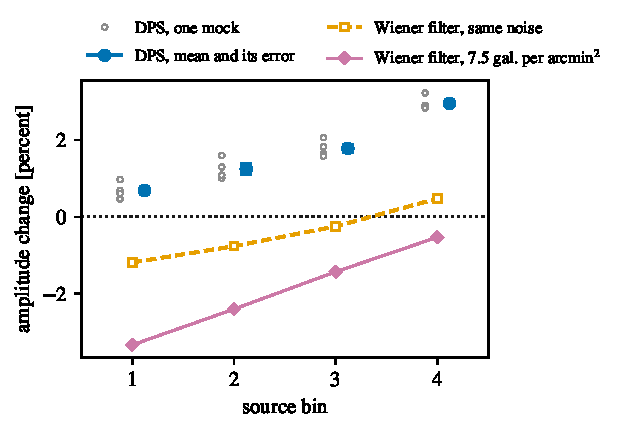
\includegraphics[width=3.5in]{plots/dps_response/dps_response.pdf}
  \caption{Change of the amplitude of the reconstructed map when the forward model ignores IA,
  per source bin, in percent of the amplitude with IA modelled. Open gray circles: DPS, one
  mock; blue circles: DPS, mean and standard error; orange open squares, dashed: tomographic
  Wiener filter at the same noise; purple diamonds: the same filter for a deeper survey;
  dotted: no change. The single-bin estimates quoted in the text are not drawn.}
  \label{fig:response}
\end{figure}

\begin{figure}[tbp]
  \centering
  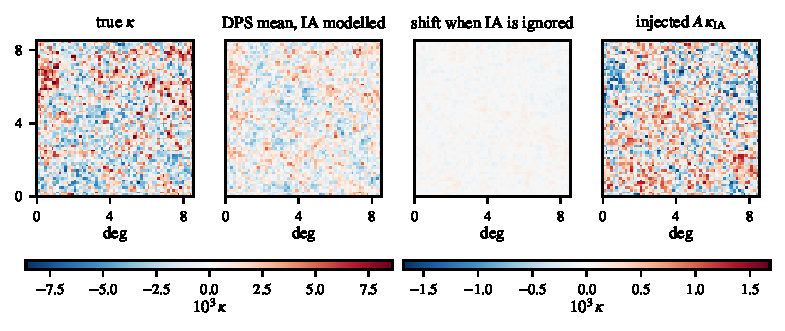
\includegraphics[width=6.2in]{plots/maps/maps.pdf}
  \caption{Source bin 1 of one mock. From left to right: the true $\kappa$; the DPS posterior
  mean with the IA model; the posterior mean with IA ignored minus with IA modelled, for the
  same data and random seed; the injected $\AIA\kIA$. The first two panels share one color
  scale and the last two share another.}
  \label{fig:maps}
\end{figure}

\appendix

\section{Method details}
\label{app:method}

\paragraph{Shell statistics.}
$\delta_i = \lambda_i\left(e^{g - \sigma_g^2/2} - 1\right)$ with $g$ a Gaussian field whose
correlation function is $\xi_g = \ln\left(1 + \xi_\delta/\lambda_i^2\right)$, so the spectrum
of $\delta_i$ is $C_i(\ell)$ for any $\lambda_i$. $\lambda_i = 1$ is the ordinary lognormal. At
\PixArcmin\ arcmin pixels the nearest shells have a pixel variance of up to \ShellVarMax, where an
ordinary lognormal puts single pixels at a $\kappa$ two orders of magnitude above the rms; the min-max normalization of the diffusion prior then compresses the signal into a
few percent of its range, a problem that is unrelated to IA. The maps use
$\lambda_i = \max(1,\, 2\,{\rm rms}(\delta_i))$, which caps the variance of $e^{g}$ and leaves
every two-point function unchanged. \NShellsShifted\ of the \NShells\ shells have
$\lambda_i > 1$; those are a statistical model and not a physical density.

\paragraph{Why the spectra come from one quadrature.}
$R$ contains $[\Ckk]^{-1}$, and the four lensing maps are strongly correlated, so $\Ckk$ is
ill conditioned. Spectra integrated pair by pair to a relative $10^{-4}$ leave the joint
covariance of $(\kappa, \kIA)$ slightly indefinite, and the inverse amplifies that: for the
eight Roman source bins the prediction $R\kappa$ built from such spectra carries spurious power
of up to \RomanSpuriousMax\ times $\CII$. Writing every spectrum as a sum over the same shells,
$C^{XY}_{ab} = \sum_i x_{a,i}\,y_{b,i}\,C_i$, makes the joint covariance a Gram matrix,
positive semi-definite to round-off, and $R$ a least-squares projection of the IA weights on
the lensing weights (\texttt{make\_ia\_spectra.py}, default method).

\section{Numerical checks}
\label{app:checks}

\begin{itemize}
  \item Shell weights against CCL: the shell sums reproduce the continuous Limber spectra
        $\Ckk$, $\CIk$, $\CII$ to \ShellsVsCCLDes\ percent for the four DES Y3 bins and \ShellsVsCCLRoman\ percent for the
        eight Roman bins (\texttt{validate\_nla\_shells.py}).
  \item Maps against their spectra: measured $\Ckk$, $\CIk$, $\CII$ of the \NTest\ held-out
        maps agree with the shell spectra within \SpectraDevHighEll\ percent for $\ell > 150$;
        the lowest multipole bins have few modes and scatter by up to \SpectraDevLowEll\ percent.
  \item Error bar of the amplitude: the pull $(\hat A - \AIA)/\sigma_A$ over ten noise
        realizations of each held-out map has width \PullWidth.
  \item Forward model: with $\AIA = 0$ the patched code returns bit-identical shear to the
        original; the DPS gradient, the pi-GDM and TDS samplers and the IA injection all run
        on CPU and on Apple MPS (\texttt{smoke\_test\_local.py}), for 4 and for 8 source bins.
  \item Toy run with IA injected by the sampler's own model (a self-consistency test,
        $\AIA = \AInjected$): $\hat A = \ToyAmpTruth \pm \ToyAmpTruthSd$ given the true map, and \ToyAmpModelled\ and
        \ToyAmpIgnored\ on the samples of the runs with and without the model, the same
        pattern as in the DES Y3-like run.
\end{itemize}

\section{Where the code and results are}
\label{app:code}

The DPS code is \texttt{Supranta/DPS\_mass\_mapping}, branch \texttt{better\_dps}, with the IA
patch, on the local branch \texttt{ia-forward-model} in \texttt{\textasciitilde/cocoa/dps\_mass\_mapping}
(\texttt{LOCAL\_SETUP.md} there lists every change). This repository holds the test:

\begin{center}
  \footnotesize
  \begin{tabular}{ll}
    \toprule
    result & script $\rightarrow$ output \\
    \midrule
    maps, shell spectra & \texttt{des\_y3\_like/make\_des\_like\_maps.py} $\rightarrow$ \texttt{work/} \\
    prior & \texttt{train.py des\_y3\_like/des\_like.yaml} $\rightarrow$ \texttt{work/results/model-1.pt} \\
    model test & \texttt{des\_y3\_like/validate\_ia\_model.py} $\rightarrow$ \texttt{results/validate\_ia\_model.json} \\
    DPS runs & \texttt{des\_y3\_like/run\_des\_like.py} $\rightarrow$ \texttt{work/samples/mock\_j.npz} \\
    DPS statistics & \texttt{des\_y3\_like/analyze\_dps.py} $\rightarrow$ \texttt{results/dps\_ia.json} \\
    figures & \texttt{notes/des\_y3\_like\_ia/plots/make\_figure\_data.py} $\rightarrow$ \texttt{plots/*/data.json} \\
    numbers & \texttt{notes/des\_y3\_like\_ia/make\_numbers.py} $\rightarrow$ \texttt{numbers.tex} \\
    \bottomrule
  \end{tabular}
\end{center}

\texttt{work/} (maps, checkpoint, samples) is not in the repository; the scripts regenerate it.
On the M3 (Apple MPS) training took \TrainMinutes\ minutes and each posterior run of four
samples about \SampleMinutes\ minutes.

\section{Open issues}
\label{app:open}

\begin{itemize}
  \item \textbf{Not real data, not $N$-body.} The shells are lognormal with bounded skewness at
        \PixArcmin\ arcmin pixels. A test on DES Y3 data requires the prior trained on the
        simulation patches at 2 arcmin and the DES Y3 shear patches, neither of which is on
        this machine.
  \item \textbf{Small sample.} \NMocks\ mocks with \NSamples\ posterior samples each. Sharing the random numbers makes the difference between the two runs precise, but the absolute correlations and slopes are those of a four-sample mean on four patches.
  \item \textbf{DPS against the Wiener filter.} The amplitude change of DPS is positive in
        every bin while the tomographic Wiener filter gives a negative change in bins 1 to 3,
        and the DPS response to the true signal is about three quarters of the Wiener one. The
        guidance of DPS is an approximation to the posterior and its strength was not
        calibrated; whether the difference comes from the guidance, from the prior, or from
        the non-Gaussianity of the maps was not separated.
  \item \textbf{The stochastic part is not in the likelihood.} $\epsilon$ carries
        \ResidFracFour\ percent of the IA variance of bin 4. Adding $S$
        to the noise of a Fourier-space likelihood, or sampling $\epsilon$ as a latent field,
        is not implemented in the sampler.
  \item \textbf{The amplitude is fixed.} Both runs use a fixed $\AIA$. Equation
        (\ref{eq:amp}) gives the conditional needed to sample it together with the maps; that
        loop is not implemented.
  \item \textbf{Prior quality.} The prior was trained for \TrainSteps\ steps. The comparison between
        the two runs is differential, but the absolute response of the posterior mean depends
        on the prior and on the guidance schedule, which were not tuned.
  \item \textbf{NLA only.} The model covers E-mode IA that is linear in the density. TATT
        terms and their B-modes are not covered.
\end{itemize}

\end{document}
